%%%%%%%% ICML 2025 EXAMPLE LATEX SUBMISSION FILE %%%%%%%%%%%%%%%%%

\documentclass{article}

% Recommended, but optional, packages for figures and better typesetting:
\usepackage{microtype}
\usepackage{graphicx}
\usepackage{subfigure}
\usepackage{booktabs} % for professional tables
\usepackage{float}

% hyperref makes hyperlinks in the resulting PDF.
% If your build breaks (sometimes temporarily if a hyperlink spans a page)
% please comment out the following usepackage line and replace
% \usepackage{icml2025} with \usepackage[nohyperref]{icml2025} above.
\usepackage{hyperref}

% Attempt to make hyperref and algorithmic work together better:
\newcommand{\theHalgorithm}{\arabic{algorithm}}

% Use the following line for the initial blind version submitted for review:
%\usepackage{icml2025}

% If accepted, instead use the following line for the camera-ready submission:
\usepackage[accepted]{packages/icml2025}

% For theorems and such
\usepackage{amsmath}
\usepackage{amssymb}
\usepackage{mathtools}
\usepackage{amsthm}

% if you use cleveref..
\usepackage[capitalize,noabbrev]{cleveref}

%%%%%%%%%%%%%%%%%%%%%%%%%%%%%%%%
% THEOREMS
%%%%%%%%%%%%%%%%%%%%%%%%%%%%%%%%
\theoremstyle{plain}
\newtheorem{theorem}{Theorem}[section]
\newtheorem{proposition}[theorem]{Proposition}
\newtheorem{lemma}[theorem]{Lemma}
\newtheorem{corollary}[theorem]{Corollary}
\theoremstyle{definition}
\newtheorem{definition}[theorem]{Definition}
\newtheorem{assumption}[theorem]{Assumption}
\theoremstyle{remark}
\newtheorem{remark}[theorem]{Remark}

% Todonotes is useful during development; simply uncomment the next line
%    and comment out the line below the next line to turn off comments
%\usepackage[disable,textsize=tiny]{todonotes}
\usepackage[textsize=tiny]{todonotes}

% The \icmltitle you define below is probably too long as a header.
% Therefore, a short form for the running title is supplied here:
\icmltitlerunning{Submission and Formatting Instructions for ICML 2025}

\begin{document}

\twocolumn[
  \icmltitle{Access Controls Will Solve the Dual-Use Dilemma}

  % It is OKAY to include author information, even for blind
  % submissions: the style file will automatically remove it for you
  % unless you've provided the [accepted] option to the icml2025
  % package.

  % List of affiliations: The first argument should be a (short)
  % identifier you will use later to specify author affiliations
  % Academic affiliations should list Department, University, City,
  % Region, Country
  % Industry affiliations should list Company, City, Region, Country

  % You can specify symbols, otherwise they are numbered in order.
  % Ideally, you should not use this facility. Affiliations will be numbered
  % in order of appearance and this is the preferred way.
  \icmlsetsymbol{equal}{*}

  \begin{icmlauthorlist}
    \icmlauthor{Evžen Wybitul}{eth}
  \end{icmlauthorlist}

  \icmlaffiliation{eth}{ETH Zurich, Switzerland}

  \icmlcorrespondingauthor{Evžen Wybitul}{wybitul.evzen@gmail.com}

  % You may provide any keywords that you
  % find helpful for describing your paper; these are used to populate
  % the "keywords" metadata in the PDF but will not be shown in the document
  \icmlkeywords{Gradient Routing, Modularization, AI Safety,
  Unlearning, Access Control, Technical AI Governance}

  \vskip 0.3in
]

% this must go after the closing bracket ] following \twocolumn[ ...

% This command actually creates the footnote in the first column
% listing the affiliations and the copyright notice.
% The command takes one argument, which is text to display at the
% start of the footnote.
% The \icmlEqualContribution command is standard text for equal contribution.
% Remove it (just {}) if you do not need this facility.

%\printAffiliationsAndNotice{}  % leave blank if no need to mention
% equal contributiono
\printAffiliationsAndNotice{} % otherwise use the standard text.

\begin{abstract}
  AI safety systems face a dual-use dilemma.
  The same request can be either harmless or harmful depending on who made it and why.
  Thus, if the system makes decisions based solely on the request's content, it will refuse some legitimate queries and let harmful ones pass.
  To address this, we propose a conceptual access control framework, based on verified user credentials (such as institutional affiliation) and classifiers that assign model outputs to risk categories (such as advanced virology).
  The system permits responses only when the user's verified credentials match the category's requirements.
  For implementation of the model output classifiers, we introduce a theoretical approach utilizing small, gated expert modules integrated into the generator model, trained with gradient routing, that enable efficient risk detection without the capability gap problems of external monitors.
  While open questions remain about the verification mechanisms, risk categories, and the technical implementation, our framework makes the first step toward enabling granular governance of AI capabilities: verified users gain access to specialized knowledge without arbitrary restrictions, while adversaries are blocked from it.
  This contextual approach reconciles model utility with robust safety, addressing the dual-use dilemma.
\end{abstract}

\section{Introduction} \label{section:introduction}

User requests --- and with them, model outputs --- exist on a
spectrum from clearly benign to clearly harmful, with most falling in
the grey zone in the middle (example in \cref{figure:main}). In the
grey zone, the same output could be considered harmful or harmless,
depending not on its content, but on its \emph{real-world context}:
who requested it and for what purpose.

\begin{figure}[t]
  \vskip 0.2in
  \begin{center}
    \centerline{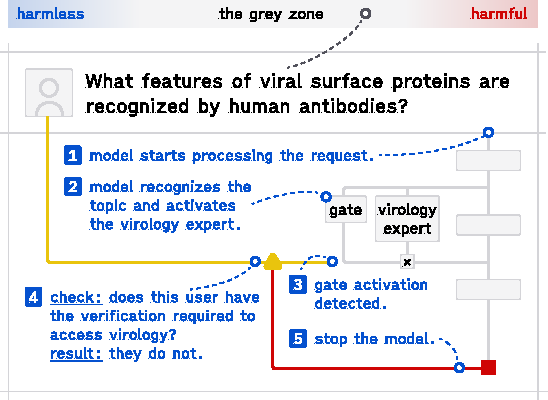
\includegraphics[width=\columnwidth]{assets/main_figure.pdf}}
    \caption{
      The user is asking a question from the grey zone: a question that could be either harmless or harmful, depending on its real-world context.
      The schema shows how the system we propose would handle it.
      (1)~The model is trained to be helpful and begins to answer the question.
      (2)~During the forward pass, the model activates its virology expert module because it is relevant to the question.
      (3)~The activation of the expert is observed by an external mechanism that immediately (4)~checks in the company's database if the user has the required authorization to access virology knowledge.
      (5)~Since they don't, the model is stopped.
    If they did, the model would be allowed to give an answer.}
    \label{figure:main}
  \end{center}
  \vskip -0.2in
\end{figure}

Safety systems that rely solely on content analysis immediately face
the \emph{dual-use dilemma}. Since the same request can be either
harmless or harmful depending on the context, wherever they draw the
refusal line, they will restrict model utility for legitimate users
while letting slip harmful requests from adversaries. Some safety
systems try to address this by considering real-world context
alongside content. However, they typically infer the context from the
content itself, making it easy for adversaries to fabricate.

In this paper, we argue that informative, hard-to-fabricate
real-world context could be obtained using user-level verifications
such as institutional affiliation, or know-your-customer checks. We
then address the dual-use dilemma with two contributions:
\begin{enumerate}
  \item We show how this type of context could be used jointly with content analysis in a safety system based on access controls \cite{butler1974}. First, generated content would be classified into risk categories. Then, a check would be performed to see whether the user has the verifications required to access the detected categories.
  \item We propose a novel technical approach to risk
    category classification that is based on gradient routing \cite{cloud2024gradientroutingmaskinggradients}. Our proposal avoids having the capability gap between a model and its monitors that can make output monitoring methods non-robust \cite{jin2024jailbreakinglargelanguagemodels}.
\end{enumerate}

Our framework is a first step toward solving the challenge of ``detection and authorization of dual-use capability at inference time'' that was highlighted by a recent survey of problems in technical AI governance \cite{reuel2025openproblemstechnicalai} and also raised by the \citet{NIST_AI_800_1_ipd_2024}.
As such, it has important governance implications, potentially enabling a more nuanced regulatory approach where access to powerful AI capabilities is stratified rather than binary, with policies that differentiate between user types and user contexts rather than focusing solely on model capabilities.
The choice of appropriate verification mechanisms and risk categories remains for future work and should ideally happen jointly with stakeholders from academia, AI governance, and industry.
Nevertheless, our approach offers a promising direction for addressing the dual-use dilemma.

\section{Current Safety Methods Don't Solve the Dual-Use Dilemma}
\label{section:current-methods}

We evaluate three AI safety approaches to see how sensitive they are
to contextual information, and whether their sources of real-world
context are trustworthy --- that is, hard to manipulate by an adversary.

% TODO Point to atual numbers of how big of a problem this is (recent paper)

First, to illustrate the need for context, consider decomposition
attacks \cite{glukhov2023llmcensorshipmachinelearning,
glukhov2024breachthousandleaksunsafe}: transforming a clearly harmful
query, such as ``How to modify a virus to avoid immune detection?'',
into a series of mundane technical questions, like the ``What
features of viral surface proteins are recognized by human
antibodies?'' from \cref{figure:main}. Here, the attacker exploits
the dual-use dilemma, and the fact that model providers cannot refuse
grey zone requests to preserve model utility.

\subsection{Unlearning: Non-Contextual Removal of Concepts}

Unlearning methods aim to remove specific knowledge, concepts, or
capabilities from a model after training
\cite{liu2024rethinkingmachineunlearninglarge}. Their goal is to
eliminate the model's ability to generate harmful content while
preserving other capabilities.

Unlearning faces significant technical challenges even for preventing behaviours that are clearly harmful.
As noted by \citet{cooper2024machineunlearningdoesntthink} and \citet{barez2025openproblemsmachineunlearning}, capabilities are hard to define, hard to remove without side effects, and it is hard to trace them back to specific data points.
Many unlearning approaches mask rather than truly remove the targeted knowledge \cite{deeb2025unlearningmethodsremoveinformation}.
Moreover, even nascent robust unlearning methods \cite{cloud2024gradientroutingmaskinggradients,lee2025distillationrobustifiesunlearning} are not contextual, and thus don't address the dual-use dilemma without additional assumptions.

\subsection{Safety Training: The Model Reacts to Context}

Safety training methods modify the model's training process to align
its outputs with human preferences.
This category includes safety pre-training \cite{maini2025safetypretraininggenerationsafe}, RLHF \cite{christiano2023deepreinforcementlearninghuman}, and safety finetuning.

Unlike unlearning, these methods are contextual.
They don't remove capabilities entirely but train the model to selectively deploy them based on, among other things, the perceived legitimacy and harmlessness of the request.
However, these qualities are entirely inferred from content supplied by the user, such as the request content, the chat history, or the model's memories about past conversations.
It should be no surprise, then, that models are susceptible to attacks that fabricate in-chat context \cite{zeng2024johnnypersuadellmsjailbreak}, or attacks that diminish models' sensitivity to in-chat context, e.g. through multi-round escalation \cite{russinovich2025greatwritearticlethat}.
Without access to trustworthy real-world context of the request, the model cannot make truly informed decisions about grey zone requests, and thus cannot robustly address the dual-use dilemma.

\subsection{Post-Processing: External Systems React to Context}

Post-processing methods are systems that classify user inputs and model outputs for the purposes of steering the underlying model, and monitoring and filtering its outputs.
Sometimes, these methods are used for usage monitoring, as is the case with Anthropic's Clio \cite{tamkin2024clioprivacypreservinginsightsrealworld, handa2025economictasksperformedai}, other times, they are used for safety, as with Llama Guard \cite{inan2023llamaguardllmbasedinputoutput} and Constitutional Classifiers \cite{sharma2025constitutionalclassifiersdefendinguniversal}.
However, similarly to safety training, the ``real-world'' context these methods work with is currently inferred mostly from user-supplied content and is thus untrustworthy and vulnerable to attacks, as evidenced by the many jailbreaks that successfully target current production systems \cite{zhang2025outputconstraintsattacksurface}.
Nevertheless, these methods could be modified to incorporate external contextual information, potentially serving as a foundation for more trustworthy, contextual safety mechanisms. We discuss this option in \cref{section:gradient-routing}.

\section{Access Controls are a Feasible Solution}
\label{section:access-controls}

In the previous section, we established that current safety systems
do not address the dual-use dilemma because they either do not
consider the real-world context of the request, or they obtain the
context directly from unverified, user-supplied content, making them vulnerable
to adversarial attacks. In this section, we present an alternative
safety framework based on access controls that directly addresses the
dual-use dilemma, and discuss some of its practical considerations.

\subsection{Overview of the Access Control Framework}

To address the problems of current safety methods, we first need a trustworthy source of real-world context about the request, or at least, about the user who made it.
Drawing inspiration from other industries, we believe we can obtain this context through user-level verification mechanisms.
These verifications could range from basic identity confirmation, to institutional affiliation, to thorough know-your-customer checks, each granting different access permissions (for more details, see \cref{section:access-controls-future-work}).

Having obtained trustworthy real-world context, we can now address the dual-use dilemma.
We propose building an access control system:
(1) define multiple risk categories such as engineering pathogens or dangerous chemicals;
(2) whenever the model is generating content, check whether it belongs to one of the risk categories, for example with the help of output classifiers (see \cref{section:risk-classification});
(3) if the user does not have the verification required for generating content in that category, take appropriate action, such as refusing the request.

This system is defensive.
Potentially harmful grey-zone requests are refused by default --- they are answered only if the user has the appropriate verifications.

Irrespective of the exact implementation, on a high level, we anticipate the system would be set up to operate as follows:

\begin{enumerate}
  \item Clearly harmless, everyday queries would require no verification, maintaining frictionless access for common use cases.
  \item Grey-zone requests would require verification that scales with potential harm. The verification requirements would be publicly available, enabling users to obtain necessary credentials ahead of time. Verification for light-grey queries would be light-weight and only used for enhanced logging, while darker-grey requests would demand progressively more stringent procedures. High-risk requests that have legitimate uses but are nevertheless currently being refused for safety reasons could still be served under the new system, if the user undergoes comprehensive verification.
  \item Finally, on the clearly harmful side, the system would still refuse the request outright.
\end{enumerate}

A system set up in this way creates a dual benefit compared to the status quo: enhanced safety through controlled access to grey-zone capabilities that deny the possibility of decomposition attacks, and expanded utility by unlocking previously restricted functionality for verified users.

\subsection{Practical Considerations for Implementation}
\label{section:access-controls-future-work}

While we cannot provide a comprehensive plan for the implementation, we outline some practical considerations below, to demonstrate the feasibility of the approach.

\paragraph{Verification} Developers will leverage existing verification infrastructure, as they do not have the expertise to build their own.
They will have to consult domain experts to find systems that are internationally standardized, globally available, and respect privacy.

Even though verification levels will differ for different fields, we expect them to follow a general template: no verification for the lowest tier, ID-based or institutional verifications for low-risk tiers, and comprehensive verifications based on existing certification infrastructure for high-risk tiers.

% TODO Verify number
For ID-based and institutional verification, established systems like KYC services and ORCID are global, standardized, low friction, and cost approximately \$1 per user [reference at least one provider].
These will help developers keep an audit trail of who has access to which potentially dangerous capabilities.

For high-risk tiers, developers can leverage domain-specific certifications that indicate a user's ability to handle dangerous information responsibly.
For example, access to information about aerosolization techniques of biological agents might require government certification for biosafety level 3, while access to information about membrane protein modification might require biosafety level 4 [cite].
While not a perfect match, these indicate the necessary safety training, equipment, and background checks.
Similar approaches apply to chemistry, where safety certifications could restrict access to laboratory protocols for producing dangerous chemicals.
% These certifications are only loosely standardized internationally, but developers can map comparable systems across countries after consulting experts; for example, BSL-3 in the US roughly corresponds to CL-3 in the EU.

This approach faces two key limitations.
First, developing countries may lack advanced certification infrastructure, potentially preventing access to knowledge.
This is a challenge that requires international cooperation.
Second, existing certifications may be overly broad for our needs.
For example, biosafety certifications verify physical equipment for handling pathogens, which is overly strict for our simpler use case of restricting access to knowledge.
We concede that the existing certification systems are just an imperfect proxy, but we believe they would be iteratively refined as the technology matures.
We also note that current legislation like the EU AI Act [cite] favours broad capability restrictions for high-risk domains, which means that our system, however imperfect, might enable access for at least some users where there would be none under the status quo.

\textbf{Risk categories} must balance granularity with technical feasibility, reflecting usage patterns, potential harm, classification reliability, and the friction of their assigned verification level.
We expect different fields of knowledge to have 1--4 risk categories, with their exact number and definition depending on the field.
In many fields, there are already standardized risk categories for physical goods (chemicals, organisms, equipment) that experts could likely map to risk categories for information (producing harmful chemicals, editing harmful organisms, operating dangerous equipment).
Initially, content could fall into two risk categories.
Standard content (requiring no verification) includes general programming and everyday queries.
High-risk content (requiring institutional verification) includes: advanced bioengineering, chemical synthesis, and advanced cybersecurity (e.g., beyond the most basic textbooks).
These categories represent specialized knowledge with clear misuse potential yet legitimate research applications.

\textbf{System responses} can vary based on risk category and classification confidence.
The initial implementation might use a three-phase response system:
(1) for outputs belonging to a risk category with high-confidence, immediate refusal with a specific explanation of the verification required;
(2) for borderline classifications, continued generation with enhanced logging and post-processing review;
(3) for verified users, seamless access with background logging for audit purposes.

\subsection{Analysis of Feasibility}

% The false positive argument is actually quite strong:
%   1.  Empirical baseline: Uses existing Anthropic classifier data (0.5% for biology)  2.  Conservative bound: Even blocking ALL biology stays under current friction tolerance  3.  Actual implementation: Will block much less than all biology  4.  Strict improvement: Expands request space in both safety and utility directions  5.  Tiered approach: Can adjust verification requirements to risk level
% The argument chain holds together well. The author successfully shows that even a very conservative upper bound (blocking all biology) results in acceptable friction levels, and the actual system would have much lower friction while providing both safety and utility improvements.

\textbf{User friction analysis}.
\begin{itemize}
  \item Access controls introduce friction from two sources: intentional verification requirements for grey-zone requests and accidental false positives from imperfect classification.
  \item By design, all grey-zone requests require verification even with perfect classifiers. Additionally, classification errors may incorrectly flag clearly harmless requests (e.g., high-school biology as advanced virology).
    % TODO Actually measure whether it is 0.5%
  \item To understand the combined impact, consider that only 0.5\% of requests involve biology topics according to Anthropic usage data.
    % TODO Mention that this comparison is a bit stretched because the companies tolerate 1% spread over all users, not concentrated into a very small user base
  \item Even if ALL biology requests required verification—an extreme upper bound—this would affect fewer users than current system friction. Existing safety systems refuse 1--7\% of benign requests as false positives, with Claude achieving the best rate of 0.4\%. Requiring verification for all biology (0.5\%) would approximately double Claude's friction rate.
  \item Additionally, verification friction differs qualitatively from current false positives—users can resolve issues through one-time credential verification rather than facing permanent refusal.
  \item Companies can calibrate friction through multiple mechanisms: adjusting grey-zone boundaries, tuning classifier thresholds, and implementing graduated responses (requesting clarification, additional context, or secondary review) rather than immediate verification requirements.
  \item Companies can determine optimal settings empirically through: (1) internal red-team decomposition attacks on concerning capabilities, (2) gradual rollout with logging to measure user impact, and (3) iterative adjustment based on safety-friction tradeoffs.
\end{itemize}

\textbf{Developer incentives for adoption}.
\begin{itemize}
    % TODO Note that this is speculative, and based on current data, companies don't tend to do this kind of differentiation
    % However, also note that there is some specialization in the companies, and with increasing model capabilities, the pressure might be higher (as the models will finally have some advanced capabilities that some companies would be willing to pay for, but enabling them generally would be too risky, and having multiple models too costly)
    % On capability ceilings: Can they provide evidence that companies are actually constrained by safety concerns from deploying valuable capabilities? Examples of "dark-grey" capabilities that labs want to offer but can't?
  \item Access controls enable competitive advantages by allowing companies to serve ``dark-grey'' requests that competitors refuse for safety reasons, while adding surgical restrictions to ``light-grey'' requests vulnerable to decomposition attacks.
    % TODO Note that this is also speculative, or maybe drop this altogether.
  \item Without access controls, continued decomposition attack success will likely trigger broad government regulations restricting model capabilities entirely.  Surgical access controls allow compliance with safety requirements while preserving advanced capabilities for verified users, creating market differentiation.
    %TODO: Add brief discussion of industry coordination mechanisms from financial KYC/content moderation precedents, e.g. through standard-setting organizations
    % TODO Add that governments might also incentivize safety through e.g. standard-setting organizations; then, having the left dial as left as possible would also be rewarded (in addition to having the right dial as right as possible)
    % TODO Dual incentive structure: Combining competitive advantage (carrot) with regulatory pressure (stick) is more robust than relying on either alone.
    % How well can they map the incentive structures? KYC was largely regulatory mandate, not voluntary adoption. Content moderation was driven by advertiser pressure. What's the analogous pressure here?
  \item Even without perfect industry coordination, first movers gain competitive advantages in serving previously restricted capabilities.
    %TODO: Acknowledge that implementing robust access controls requires significant company investment in verification infrastructure; this could be mitigated through government grants that would e.g. require the verification infra to be open-sourced, thus shared with other companies.
    % On government incentives: This might be the strongest part - if governments reward safety through standard-setting organizations, companies have clear incentives to adopt the most restrictive approach possible while maintaining utility.
    % Govs do not want to stifle innovation but also want to enable safety; they should recognize that they will need to issue more than blanket bans on capabilities. Currently, they don't have good tools to do so, but with access controls, they would — and they would use them.
\end{itemize}

\paragraph{Privacy concerns}.

\section{Implementing Risk Classification} \label{section:risk-classification}

A core requirement of the verification-based access control system
described in \cref{section:access-controls} is being able to reliably
classify model outputs into risk categories.
This classification needs to address key challenges: accuracy with
minimal false positives, resistance to adversarial attacks, and efficiency.
We examine two approaches to implementing this classification --- one
currently available and one theoretical --- and discuss their trade-offs.

\subsection{Post-Processing}

As discussed in \cref{section:current-methods}, current systems
already rely on post-processing classifiers that analyse outputs
before delivery to users.
These could be adapted for content classification into risk
categories in an access control system.
For example, a classifier could be trained to identify moderately
advanced virology topics and, if detected, could trigger verification
of user permissions before delivering the output.

The key advantage of post-processing systems is modularity, as they
can be developed and updated independently of the generation models
they oversee.
However, they face a trade-off between usability (latency) and safety
\cite{kumar2025freelunchguardrails}: prioritizing low latency can
create a capability gap between generators and monitors that
sophisticated language models can exploit
\cite{jin2024jailbreakinglargelanguagemodels}.
Despite this limitation, recent post-processing methods show
acceptable efficiency and resilience toward jailbreaks
\cite{sharma2025constitutionalclassifiersdefendinguniversal} and
could provide a practical initial implementation path for
output-based access control.

\subsection{Gradient Routing} \label{section:gradient-routing}

To address the capability gap problem in post-processing methods, we
detail how gradient routing \cite{cloud2024gradientroutingmaskinggradients}
could be adapted to classify model outputs into risk categories.
Our adaptation represents a theoretical direction for integrating
risk category detection directly into model architecture.
This approach can be combined with post-processing methods and offers
different trade-offs.

We propose augmenting models with small expert modules controlled by
learned gates, as shown in \cref{figure:main}.
During model training, assuming we have examples from the relevant
risk categories (e.g., advanced virology), the expert module would be
made to receive gradients exclusively from these examples.
Simultaneously, the module's gate would be trained to activate the
module on these examples using an auxiliary loss function.
We hypothesize this would lead to the module obtaining specialist
knowledge from the risk domain, and to the model learning to activate
the module whenever this knowledge is needed.

\Cref{figure:main} illustrates this in the context of the wider
access control system: when a user requests information about viral
surface proteins, the model correctly recognizes the domain and
activates the virology gate, engaging the expert but also triggering
the verification system. If the user lacks appropriate credentials,
the system takes the appropriate response --- here, halting the generation.

This approach eliminates the efficiency-capability
trade-off inherent in post-processing methods: the risk category
classifier is embedded within the larger model, so there is no
capability gap, and because the gated module is small and integrated
into the model's forward pass, it is computationally efficient with
minimal impact on latency.

Crucially, during standard training, the model is naturally incentivized to identify risk category information in inputs and surface this in its representation space, as this is directly linked to enabling the right specialized module at the right time.
This approach differs fundamentally from post hoc methods like probing or sparse autoencoders \cite{cunningham2023sparseautoencodershighlyinterpretable}, which cannot guarantee the model actually operates with the concepts they attempt to identify.

Additionally, it resolves the adversarial dynamic (model vs. monitors, helpful vs. harmless) common in AI safety by aligning training incentives with safety objectives.

Several technical challenges remain.
While gradient routing has shown promise in creating specialized modules in smaller models, its effectiveness in larger language models, particularly with the gated-expert architecture, requires empirical validation.
Other key challenges include preventing false positives and false negatives, though regularization techniques and adjusted detection thresholds, respectively, could mitigate these issues.

% TODO Better explain why FT is useful
Our approach also requires identifying risk categories during initial training, prompting research into adaptation of gradient routing for fine-tuning scenarios.
Despite these challenges, the approach offers promising theoretical properties that warrant experimental investigation.

\section{Conclusion}

We argued that safety systems that do not utilize contextual
information face a lose-lose \emph{dual-use dilemma}: they will
restrict model utility for some legitimate users while still allowing
some adversaries to use the model for ill. To address this problem,
we introduced a new access control framework that limits access to
outputs from certain risk categories only to users with relevant
verifications (which serve as proxies for trustworthy real-world
context). We also proposed a novel technical solution for classifying
outputs into risk categories based on gradient routing that has the
potential to resolve the efficiency-robustness trade-off of
post-processing methods.

Beyond addressing specific technical challenges, our framework
represents a promising governance shift from working with model-level
abstractions and binary capability restrictions toward more granular
user-level access controls. This offers a practical pathway for
regulating increasingly powerful AI systems through stratified access
rather than blanket capability limitations.

\section*{Acknowledgements}

We thank Jakub Kryś, Dennis Akar, and Kola Ayonrinde for their feedback on a draft of this paper. We thank Joseph Miller, Alex Cloud, Alex Turner, and Jacob Goldman-Wetzler for discussions on gradient routing.

\bibliography{references}
\bibliographystyle{packages/icml2025}

%%%%%%%%%%%%%%%%%%%%%%%%%%%%%%%%%%%%%%%%%%%%%%%%%%%%%%%%%%%%%%%%%%%%%%%%%%%%%%%
%%%%%%%%%%%%%%%%%%%%%%%%%%%%%%%%%%%%%%%%%%%%%%%%%%%%%%%%%%%%%%%%%%%%%%%%%%%%%%%
% APPENDIX
%%%%%%%%%%%%%%%%%%%%%%%%%%%%%%%%%%%%%%%%%%%%%%%%%%%%%%%%%%%%%%%%%%%%%%%%%%%%%%%
%%%%%%%%%%%%%%%%%%%%%%%%%%%%%%%%%%%%%%%%%%%%%%%%%%%%%%%%%%%%%%%%%%%%%%%%%%%%%%%
\newpage
\appendix

\section{Risk Tiers and Verification Levels in Bioweapon Construction}

We provide a more detailed example of the access control system in the context of biology to illustrate a possible initial implementation of the system.
However, we stress that this is a hypothetical example, and that an actual system would be more granular and require a lot of input from experts in the field (which we are, decidedly, not).

\subsection{Tier 0: No risk}

\paragraph{Verification} No verification required. This tier contains information that is already freely available in undergraduate textbooks and poses no additional risk when accessed through AI systems.

\begin{itemize}
  \item \textbf{Standard techniques in molecular biology} including PCR amplification, DNA cloning, bacterial transformation, and gel electrophoresis. These are taught in undergraduate courses and have limited applications to building bioweapons.
  \item \textbf{Basic laboratory safety procedures}. These are fundamental to all biological work and widely available.
\end{itemize}

\subsection{Tier 1: Low risk}

Basic ID-based verification through existing providers. This is mostly to keep an audit trail matching people to requested knowledge. This approximately corresponds to the standard BSL-1 and BSL-2.

\paragraph{Verification implementation} Services like Trulioo provide global identity verification through government-issued ID documents, biometric verification, and address confirmation. These services already operate in most countries and cost approximately \$1 per verification. The integration requires standard API implementation and creates minimal operational overhead. For academic users, verification could instead utilize existing systems like ORCID (global researcher identification) or institutional email verification through services like SwiftVerify that confirm academic affiliations.

\begin{itemize}
  \item \textbf{BSL-1 and BSL-2 organism cultivation and procedures}. While BSL-2 organisms can cause disease, they're standard in medical laboratories and educational settings.
  \item \textbf{Basic CRISPR-Cas9 techniques}. These are fundamental to modern biology education and research, but could be used for dangerous modifications.
  \item \textbf{Large-scale fermentation and bioprocessing}. This is essential to biotechnology but could theoretically support harmful production.
\end{itemize}

\subsection{Tier 2: High risk}

Maximum security for knowledge with significant weapons potential and limited legitimate applications. This approximately corresponds to the standard BSL-3 and BSL-4.

\paragraph{Verification implementation} Model developers would tap into existing BSL-3/BSL-4 laboratory certification databases maintained by national authorities across major countries. In the United States, this involves accessing CDC select agent program registrations and NIH BSL-3/4 facility certification databases. In the European Union, individual member states maintain containment level (CL-3/CL-4) facility registrations that map directly to BSL levels. Canada maintains Physical Containment (PC-3/PC-4) facility databases, Australia has BSL-3/4 certification records, and Japan, China, and other major countries maintain similar systems with compatible standards. Additionally, access to high-risk knowledge might be only per-project, and each project might require approval from an expert committee.

\begin{itemize}
  \item \textbf{BSL-3 organism cultivation.} These are biological weapons agents with limited legitimate applications.
  \item \textbf{BSL-3 and BSL-4 laboratory procedures.} These require specialized facilities and training with security implications.
  \item \textbf{Specific information about toxin genes} including botulinum, ricin, and diphtheria toxin genes, the way to obtain them, work with them, and insert them into organisms. These are extremely limited in legitimate applications.
  \item \textbf{Complete viral genome synthesis techniques.} These can recreate dangerous viruses with minimal legitimate applications.
  \item \textbf{Advanced CRISPR applications} including multiplex editing and epigenome editing. These have greater potential for creating dangerous modifications and are typically used only in advanced research settings.
  \item \textbf{Cell membrane and surface protein modification techniques.} These are critical enablers for immune evasion.
  \item \textbf{Aerosol generation techniques for biological agents.} These are specifically needed for biological weapons delivery despite some pharmaceutical applications.
\end{itemize}

\end{document}

% This document was modified from the file originally made available by
% Pat Langley and Andrea Danyluk for ICML-2K. This version was created
% by Iain Murray in 2018, and modified by Alexandre Bouchard in
% 2019 and 2021 and by Csaba Szepesvari, Gang Niu and Sivan Sabato in 2022.
% Modified again in 2023 and 2024 by Sivan Sabato and Jonathan Scarlett.
% Previous contributors include Dan Roy, Lise Getoor and Tobias
% Scheffer, which was slightly modified from the 2010 version by
% Thorsten Joachims & Johannes Fuernkranz, slightly modified from the
% 2009 version by Kiri Wagstaff and Sam Roweis's 2008 version, which is
% slightly modified from Prasad Tadepalli's 2007 version which is a
% lightly changed version of the previous year's version by Andrew
% Moore, which was in turn edited from those of Kristian Kersting and
% Codrina Lauth. Alex Smola contributed to the algorithmic style files.
